\section{Missionen}
\label{sec:module.Missionen}
\begin{figure}[H]
\centering
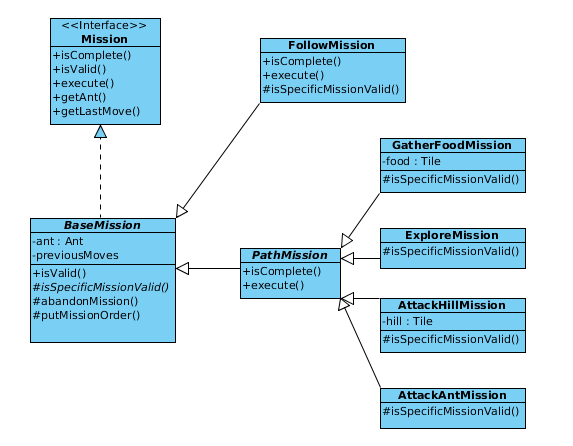
\includegraphics[width=0.9\textwidth]{91_bilder/Missions}
\caption{Missionen}
\label{fig:missions}
\end{figure}
Eine Mission dauert �ber mehrere Spielz�ge. Die meisten Missionen (GatherFoodMission, ExploreMission, AttackHillMission, AttackAntMission) sind Pfadmissionen\footnote{Die abstrakte Klasse PathMission ist im Code unter ants.missions.PathMission.java auffindbar.}, bei welchen die Ameise einem vorgegebenen Pfad, der bereits beim Erstellen der Mission berechnet wurde, folgt. 
Die FollowMission ist eine spezielle Mission, mit der eine Ameise einfach einer anderen Ameise hinterherl�uft.

Eine Mission kann auch abgebrochen werden, wenn es keinen Sinn mehr macht, sie weiter zu verfolgen. Je nach spezifischer Mission sind aber die Abbruchbedingungen anders. Zum Beispiel die GatherFoodMission ist nur solange g�ltig wie das Futter noch nicht von einer anderen Ameise eingesammelt wurde.
Abbildung \ref{fig:missions} zeigt einen \"Uberblick �ber die wichtigsten Missionen und ihre Hierarchie.
